\section*{Ziel}
Ziel des Experimentes ist die Untersuchung der äußeren Elektronenhülle von Alkali-Atomen, zu bestimmen ist die Abschirmungszahl.\\
Im Detail wird durch Spektroskopie mit sichtbarem Licht das Coulomb-Feld des Kernes an den äußeren Elektronenschalen untersucht,
welches durch die inneren Elektronenschalen von inneren Elektronen abgeschwächt ist.

\section{Theorie}
\label{sec:Theorie}
\subsection{Ein-Elektron-Systeme} % (fold)
\label{sub:1e}
%Das exakte Beschreiben des Verhaltens von angeregten Atomen, wie etwa die Wellenlänge der emittierten Strahlung, ist aufwendig.
Das verwendete Atom wird im Folgenden als Ein-Elektron-System angenommen, welches die Grundzüge des Bohrschen Atommodells des Wasserstoffs aufweist.
Sämtliche Emissions- und Absorbtionsvorgänge werden ausschließlich dem äußeren Elektron zugeschrieben, während verbliebene innere Elektronen ihren Zustand beibehalten.
Dieses äußere Elektron wird zweckmäßig Leuchtelektron genannt.

Ein wichtiger Unterschied dieser Systeme ist, dass das Leuchtelektron des Wasserstoffs nicht durch innere Elektronen beeinflusst wird.
Das Leuchtelektron des Alkali-Atoms befindet sich indes im Feld des Kernes, welches durch vorhandene innere Elektronen geschwächt wird.

\subsection{Anpassung des Modells: Kugelsymmetrie, Potential und Bahndrehimpulsquantenzahl} % (fold)
\label{sub:L_quantenzahl}
Weiterer Unterschied des Bohrschen Atommodells von Wasserstoff zu dem hier hier angenommenen Ein-Elektron-System ist die Anzahl der Spektrallinien. 
Im Kontrast zu den weitesgehend monochromatischen Linien des Wasserstoffs, wird bei Alkali-Atomen ein linienreiches Spektrum erwartet.
Dieses Spektrium weist auf weitere Quantenzahlen nebst der Hauptquantenzahl hin.

Die Elektronen des Wasserstoffs befinden sich im Zuge der Quantenmechanischen Grundlagen im gebundenen Zustand in der Atomhülle.
Ihr Zustand ist Lösung der zeitinvarianten Schrödingergleichung
\begin{equation}
	\Bigl(\Bigl(\frac{\hbar^2\mathup{\Delta}}{2 m_0}\Bigr)+U\Bigr)\psi=E\psi
	\label{eq:schroedinger}
\end{equation}
mit der potentiellen Energie 
\begin{equation}
	U=-\frac{e_0^2}{4\pi\epsilon_0 r}.
	\label{eq:Epot}
\end{equation}
Mit der Rydberg-Konstanten $R_\infty$ ergeben sich die Energieeigenwerte des Leuchtelektrons von
\begin{equation}
	E(n)=R_\infty\frac{1}{n^2}, \qquad n\in\mathbb{N}
	\label{eq:EEW}
\end{equation}
die die Energie beim Quantensprung vorhersagen.

Bei der Betrachtung des Ein-Elektron-System wird die potentielle Energie $U$ \eqref{eq:Epot} durch
\begin{equation}
	U=-\frac{e_0^2}{4\pi\epsilon_0 r}(z-\sigma)
	\label{eq:Epot_neu}
\end{equation}
ersetzt.
Dieses Potential betrachtet neben dem Leuchtelektron die Abschrimungszahl $\sigma$, die stellvertretend für die Rumpfelektronen den Einfluss zwischen Kern und Leuchtelektron dämpft.
%Zum Einen betrachtet die Schrödingergleichung \eqref{eq:schroedinger} nur noch den Impuls des Leuchtelektrons, zum Anderen wird der Hamilton-Operator im Interesse der vorliegenden Symmetrie in Polarkoordinaten umgeschrieben.
Ausnutzen der Symmetrie ergibt die angepasste Schrödingergleichung
\begin{equation}
	\biggl(\frac{\hbar^2}{2m_0}\frac{1}{r}\frac{\partial^2 r}{\partial r^2}+\frac{1}{2m_0}\frac{1}{r^2} \vec{L}^2-(z-\sigma)\frac{e_0^2}{4\pi\epsilon_0 r}\frac{1}{r}\biggr)\psi=E\psi
	\label{eq:schroedinger_2}
\end{equation}
mit dem Drehimpulsoperator $\hat{L}=-i\hbar \vec{r}\times\nabla$.

Die Lösung des Eigenwertproblem wird gesucht, indem innerhalb der Gleichung die Eigenwerte von $L$ gesucht und mit ihnen die Gleichung vereinfacht wird.
%Die Lösungen des inneren Eigenwertproblems sind Kugelflächenfunktionen $Y_l(\theta,\phi)$ mit den Eigenwerten $\hbar^2 l(l+1), l\in\mathbb{N_0}$.
Die Eigenwerte werden als Bahndrehimpulsquantenzahl $l$ bezeichnet.
Damit erscheint Gleichung \eqref{eq:schroedinger_2} als
\begin{equation}
	\biggl(\frac{\hbar^2}{2m_0}\frac{1}{r}\frac{\partial^2 r}{\partial r^2}+\frac{\hbar^2}{2m_0}\frac{1}{r^2} l(l+1)-(z-\sigma)\frac{e_0^2}{4\pi\epsilon_0 r}\frac{1}{r}\biggr)\psi_R=E\psi_R.
	\label{eq:EEW_drehimpuls_flasche}
\end{equation}
In dieser Gleichung wird die Lösung $\psi$ in Radialanteil $\psi_R$ und in Winkelanteil $\psi_W$ aufgespalten. 
Die Energieeigenwerte sind
\begin{equation}
	E=R_\infty\frac{(z-\sigma)^2}{(k+1+l)^2} \qquad k\in\mathbb{N_0}
	\label{eq:EEW_drehimpuls}
\end{equation}

%Zu erkennen ist, dass der Ausdruck $k+1+l$ der Hauptquantenzahl $n$ entspricht, welche ausschließlich die Energieeigenwert $E(n)$ bestimmen, und dass mit $l_\text{max}=n-1$ die Drehimpulsquantenzahlen $l\in\mathbb{N_0}$ nach oben beschränkt sind.

\subsection{Anpassung des Modells: relativistische Effekte} % (fold)
\label{sub:rel}
Der in Abschnitt \ref{sub:L_quantenzahl} gefundene Ausdruck \eqref{eq:EEW_drehimpuls} lässt nun analog zu \eqref{eq:EEW} Aussage über die Energie eines Leuchtelektrons zu.
Der Ausdruck \eqref{eq:EEW_drehimpuls} berücksichtigt keine relativistischen Effekte.
Diese Näherung hat zur Folge, dass die Energieeigenwerte scheinbar keine Abhängigkeit von den Drehimpulsquantenzahlen zeigen.
Unter Berücksichtigung relativistischer Effekte gilt für den Hamilton-Operator in den Schrödinger-Gleichungen
\begin{equation}
	\hat{H_\text{rel}}\approx\frac{\hat{P}^2}{2m_0}-\frac{1}{8}\frac{\hat{P}^4}{m_0^3 c^2}
	\label{eq:relativerhamilton}
\end{equation}
Es wird der relativistische Effekt als klein angenommen, in dem gefundenen Hamilton-Operator kann der zweite Term als Störungsoperator angesehen werden.

Durch die additive Anpassung des Operators bleiben die vorangegangen Energieeigenwerte im Wesentlichen erhalten.
Die relativistischen Eigenwerte sind die Eigenwerte \eqref{eq:EEW_drehimpuls} zuzüglich der Erwartungswert des Störungsoperator mit den Eigenfunktionen.
Das Ergebnis der relativistischen Anpassung ist
\begin{equation}
	E=-R_\infty\biggl(\frac{(z-\sigma)^2}{n^2}+\alpha^2\frac{(z-\sigma)^4}{n^3}\biggl(\frac{2}{2l+1}-\frac{3}{4n}\biggr) \biggr)\qquad k\in\mathbb{N_0}
	\label{eq:EEW_rel}
\end{equation}
mit der Sommerfeldschen Feinstrukturkonstante $\alpha=\frac{e_0^2}{2hc\epsilon_0}$
% subsection subsection_name (end)

\subsection{Betrachtung des Spins} % (fold)
\label{sub:spin}
%In vorangegeangen Abschnitten wurde die Schrödingergleichung \eqref{eq:schroedinger} gemäß der Symmetrie umgeformt, die potentielle Energie $U$ angepasst und mithilfe relativistischer Betrachtung eine Formel erschlossen, die die Energiewerte des Leuchtelektrons in Abhängigkeit von Hauptquantenzahl $n$ und Drehimpulsquantenzahl $l$ vorhersagt.
%Präzise experimentelle Beobachtung zeigen eine Abweichung von dieser Theorie, die durch Berücksichtigen einer weiteren Eigenschaft der Elektronen berichtigt werden kann.

Aus Experimenten wie dem Stern--Gerlach-Experiment ist eine weitere Eigenschaft, der Spin, bekannt.
Die zugehörige Quantenzahl $s$ hat nur den Betrag $\sfrac{1}{2}$.
Mit dem Drehimpuls der Elektronen geht ein magnetisches Moment einher, welches in Wechselwirkung mit anderen Elektronen tritt.
%Diese Wechselwirkung wird das Spin-Bahn-Kopplung bezeichnet.
Die Summe des aus Abschnitt \ref{sub:L_quantenzahl} bekannten Drehimpulsoperators $L$ und dem eingeführten Spinoperator $S$ ergibt die Quantenzahlen
$j=l\pm\sfrac{1}{2}$.
Der Einfluss des Spins auf die Energieeigenwerte kann als klein angenommen werden, somit wird der Effekt mit Hilfe der Störungstheorie und der Diracschen Theorie des relativistischen Elektrons ermittelt.
Die Anpassung der Energieeigenwerte erfolgt wie in Abschnitt \label{sub:rel} durch Addition des Erwartungswertes vom angepassten Hamilton-Operators in Bezug auf Eigenfunktionen.

Es ergibt sich die Energieeigenwert-Gleichung
\begin{equation}
	E=-R_\infty\biggl(\frac{(z-\sigma)^2}{n^2}+\alpha^2\frac{(z-\sigma)^4}{n^3}\biggl(\frac{1}{j+\sfrac{1}{2}}-\frac{3}{4n}\biggr) \biggr),
	\label{eq:EEW_3}
\end{equation}
die schließlich die drei Quantenzahlen $n,l,j$ berücksichtigt.
Gleichung \eqref{eq:EEW_3} stellt die Sommerfeldschen Feinstrukturformel in erster Näherung dar.

\subsection{Auswahlregeln und erwartete Lage der Spektrallinien}
Aus Experimenten ist bekannt, dass nicht alle Quantenübergänge gleich wahrscheinlich sind.
Es ergibt sich einerseits, dass Übergänge nicht auftreten, bei welchen sich der Bahndrehimpuls nicht ändert, also $\mathup\Delta l=0$, oder bei welchen sich  die Bahndrehimpulsquantenzahl um mehr als zwei ändert, also $\mathup\Delta l\ge2$.
%Mit dieser Einschränkung können nur Übergänge beobachtet werden, bei welchen sich die Bahndrehimpulsquantenzahl um eins ändert.
Andererseits ist die Änderung der Quantenzahl $j$ sehr wahrscheinlich, wenngleich $\mathup\Delta j=0$ nicht ausgeschlossen ist.

Die Energiedifferenz zwischen einer Änderung im Bahndrehimpulsquantenzahl $l$ ist groß im Vergleich zur derjenigen der Änderung in der Quantenzahl $j$.
Mit der in Abschnitt \ref{sec:Durchfuehrung} beschriebenen Vorrichtung wird der Abstand zwischen verschiedenen Bahndrehimpulsquantenzahlen groß und zwischen verschiedenen Quantenzahlen $j$ klein angenommen.
Wegen des binären Spins werden also gewissermaßen für jede Bahndrehimpulsquantenzahl $l$ zwei dicht beieinander liegende Linien erwartet, die als Dublett-Struktur bezeichnet wird.

\subsection{Betrachtung der Abschirmungszahlen \texorpdfstring{$\sigma$}{Sigma}}
Zur Abgrenzung des Ein-Elektron-Systems wurde in das Bohrsche Modell die Abschirmungskonstante $\sigma$ eingeführt, die den Einfluss der Rumpfelektronen auf das Feld des Kernes und auf das Leuchtelektron beschreibt.
Die Aufenthaltswahrscheinlichkeit des Leuchtelektrons innerhalb des Atoms ist nicht verschwindend, weshalb alle Rumpfelektronen Einfluss auf das Leuchtelektron nehmen.
Es erweist sich als sinnvoll, die Abschirmungszahl $\sigma$ in zwei Teile aufzuspalten.\\
Der erste Teil, $\sigma_1$, ist die Konstante der vollständigen Abschirmung. 
Sie nimmt mit $n,l$ und der Ordnungszahl $z$ zu und beschreibt den Einfluss aller Rumpfelektronen auf das Leuchtelektron.
Der zweite Teil, $\sigma_2$, ist die Konstante der inneren Abschirmung. 
Sie nimmt mit $n,l$ zu und ist stets kleiner als $\sigma_1$.
Die Rumpfelektronen im Inneren der Schale des Leuchtelektrons haben zusätzlichen Einfluss, anders die restlichen Rumpfelektronen außerhalb.
Die Konstante der inneren Abschirmung $\sigma_2$ berücksichtigt den Effekt der Spin-Bahn-Kopplung.

Der Unterschied zwischen den beiden Konstanten ist für Leuchtelektronen auf der äußeren Schale eines Atoms nur gering, weshalb im Folgenden die Konstante $\sigma_2$ gesucht wird.
Dies geschieht durch das Ausmessen der Energiedifferenz innerhalb der Dublett-Struktur.
Mit
\begin{equation}
	E=-R_\infty\biggl(\frac{(z-\sigma_1)^2}{n^2}+\alpha^2\frac{(z-\sigma_2)^4}{n^3}\biggl(\frac{1}{j+\sfrac{1}{2}}-\frac{3}{4n}\biggr) \biggr)
\end{equation}
folgt für die Energiedifferenz
\begin{equation}
	\mathup{\Delta}E=\frac{R_\infty\alpha^2}{n^3}(z-\sigma_2)^4\frac{1}{l(l+1)}\approx hc\frac{\mathup{\Delta}\lambda}{\lambda^2}
\end{equation}

\subsection{Kurze Einführung in Beugungsgitter}
\begin{figure}
	\centering
	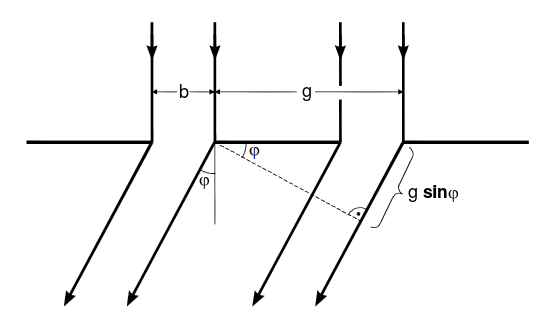
\includegraphics[width=0.7\textwidth]{Bilder/Gitter.png}
	\caption{Beugung einer ebenen Welle an regelmäßig angeordneten Spaltöffnungen der Breite $b$. \cite{skript}} 
\end{figure}
Das Beugungsgitter ist eine lichtundurchlässige Platte, in die im präzisen geringen Abstand $g$ schmale parallele Spalten der Breite $b$eingeätzt wurden.
Die Anzahl der beleuchteten Spalte ist $p$.
Die Größenordnung des Gitters bewirkt Beugungsphänomene, anhand derer die Wellenlänge des einfallenden Lichtes bestimmt werden kann.
Im Zusammenhang stehen die Wellenlänge des Lichtes und die Ablenkung.

%Für die Intensität des Lichtes in Abhängigkeit vom Ablenkungswinkel gilt bei einer Öffnung
%\begin{equation}
%	I_1(\phi)=E_0^2b^2\frac{\lambda}{\pi b\sin{\phi}}\sin^2{\frac{\pi b\sin{\phi}}{\lambda}}.
%\end{equation}

%Mit der Überlagerung mehrer Spalten wird eine Funktion der Gestalt
%\begin{equation}
%	I_2=|E(\phi)|^2\cdot I_1
%\end{equation}
%angenommen.
%Die Amplitudenfunktion $E$ ergibt sich durch die Überlagerung der Lichtstrahlen ausgehend von den Einzelspalten,
%\begin{equation}
%	E=e^{i(\omega t-2\pi \sfrac{z}{\lambda})}(1+e^{-i\delta}+e^{-i\delta}+...+e^{-(p-1)i\delta}).
%\end{equation}
%Nach Anwendung der geometrischen Reihe und Umformung durch die Eulersche Formel ergibt sich
%\begin{equation}
%	I_2(\phi)=E_0^2b^2
%	\frac{\lambda}{\pi b\sin{\phi}}
%	\sin^2{\frac{\pi b\sin{\phi}}{\lambda}}
%	\frac{\sin^2{p\pi g\sin{\phi}/\lambda}}
%	{\sin^2{\pi g\sin{\phi}/\lambda}}.
%\end{equation}
%
Typische für Beugungsbilder am Gitter sind schmale und helle Hauptmaxima.
Ihre Lage wird mit 
\begin{equation}
	\sin{\phi}= k\frac{\lambda}{g} 
	\label{eq:hauptmaxima}
\end{equation}
mit $k\in\mathbb{N_0}$ und der Gitterkonstanten $g$ abgeschätzt.
Mit Gleichung \eqref{eq:hauptmaxima} ist die Verbindung zwischen Wellenlänge und Ablenkung gegeben.

Die Auflösung des Gitterbeugungsbildes ist sehr hoch.
Die maximale Auflösung wird beschrieben durch das Verhältnis der gemittelten Wellenlänge zur Differenz der Wellenlänge
zwischer zwei Linien, die noch vom Gerät voneinander unterscheidbar sind, $A=\frac{\bar\lambda}{\Delta\lambda}$.
Zwei Linien gelten dabei als unterscheidbar, wenn das Maximum einer Linie nicht näher an das Maximum einer anderen Linie kommt als der Abstand zwischen Hauptmaximum und erstem Minimum.\\
Mithilfe der Gleichung \eqref{eq:hauptmaxima} wird die Lage des Minimums einer Linie $\lambda+\Delta\lambda$ auf das Maximum einer anderen Linie $\lambda$ gelegt und damit die Auflösung zu
\begin{equation}
	A=kp
\end{equation}
bestimmt, woraus folgt, dass die Auflösung von der Ordnung $k$ des Maximums und von der Anzahl $p$ der Gitterspalten abhängt.